\chapter{Hexagonales Schach}

Hexagonales Schach hat viele unterschiedliche Spielweisen. Diese variieren nicht nur in den möglichen Zügen, sondern auch in der Anzahl der Spielsteine und der Größe des Spielfelds. Glinskis Regeln werden für die Europameisterschaften in hexagonalem Schach genutzt \cite{Gados:Hexagonal}. In der Version von Glinski besteht das Spielbrett aus 91 Feldern, die zu einem perfekten Hexagon angeordnet werden. Dies ist nicht in jeder Schachvariante gleich. Schafran lässt die Spalten a und l aus (vgl. Abbildung \ref{fig:hex:start}). Dazu variiert noch die Startaufstellung.

\begin{figure}[H]
    \centering
    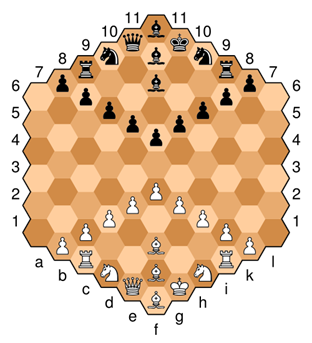
\includegraphics{images/hexStart.png}
    \caption{Startaufstellung Glinski \protect\footnotemark}
    \label{fig:hex:start}
\end{figure}
\footnotetext{\url{https://commons.wikimedia.org/wiki/Category:Glinski\%27s_hexagonal_chess}}

Glinskis Startaufstellung ist eine Raute \cite{GlinskiHexaChess}(vgl. Abbildung \ref{fig:hex:start}). McCooey füllt in seiner Version die freien Flächen auf \cite{McCoeeyHexaChess}. Turm und Pferd rücken näher zusammen und formen so eine Route aus den Figuren. Alle Bauern rücken ein Feld zurück. Die Bauern, welche danach außerhalb stehen würden, werden entfernt. In Schafrans Version werden die Figuren in einem V  aufgestellt \cite{SchafranHexaChess}. Jede Figur bekommt einen Bauern vor sich gestellt. Ein Bischof wird vom Spielbrett entfernt. Das V erstreckt sich vom linken Rand bis zum rechten Rand. 



\begin{table}[H]
    \centering
    \begin{tabular}{|c|c|}
        \hline
        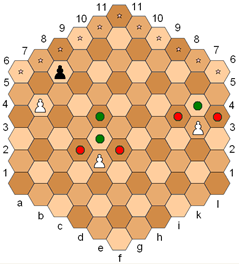
\includegraphics{images/hexPawn.png} & 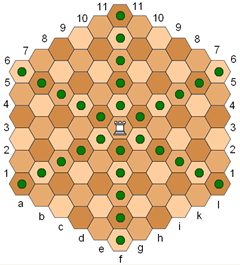
\includegraphics{images/hexRook.png} \\ \hline 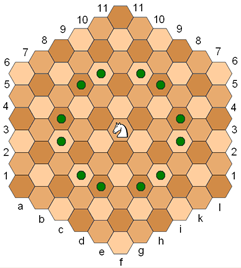
\includegraphics{images/hexKnight.png} & 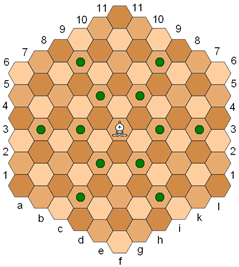
\includegraphics{images/hexBishop.png} \\ \hline 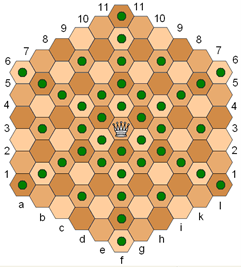
\includegraphics{images/hexQueen.png} & 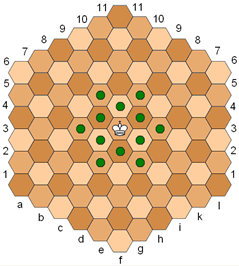
\includegraphics{images/hexKing.png} \\ \hline
    \end{tabular}
    \caption{Gültige Schachzüge in der hexagonalen Variante \protect\footnotemark}
    \label{tab:posMove}
\end{table}
\footnotetext{\url{https://commons.wikimedia.org/wiki/Category:Glinski\%27s_hexagonal_chess}}

\newpage
Der Bauer bleibt weiter die schlechteste Figur des Spiels \cite{GlinskiHexaChess}. Im Vergleich zum normalen Schach gewinnt der Bauer nicht an Zügen und Potential. Umwandlung gibt es ebenfalls im hexagonalen Schach. Das macht den Bauern zum Ende des Spiels zu einer wertvollen Figur mit Potential \cite{chessvar}. Die Distanz zum Spielfeldende ist in den Versionen gleich. (vgl. Tabelle \ref{tab:posMove})\par
Der Turm darf sich bis zum Rand in jede Richtung orthogonal, also die direkt anliegenden Felder, bewegen \cite{GlinskiHexaChess}. Spielfiguren behindern seine Bewegungsmöglichkeiten. Der Turm ist die wertvollste Figur nach der Königin. Anders als im normalen Schach ist der Turm allein nicht in der Lage einen König abzuschneiden. Dadurch, dass der König auch diagonal, über eine Linie verbundene Felder, laufen kann, werden zwei Türme benötigt. Der Turm ist im hexagonalen Schach in der Lage 1/3 des Spielfeldes abzudecken. Im herkömmlichen Schach kann der Turm nur 1/4 von dem Spielfeld abdecken. Durch seinen erweiterten Aktionsradius hat der Turm im Vergleich zur herkömmlichen Variante an Potenzial gewonnen. (vgl. Tabelle \ref{tab:posMove})
\par
Der Springer kann sich auf die Felder bewegen, welche zwei Felder orthogonal entfernt sind und danach jeweils links und rechts oben von der Ausgangsposition \cite{GlinskiHexaChess}. Drei Züge werden gebraucht, um komplett über das Feld zu kommen. Der Springer hat sich im Vergleich zum normalen Schach nicht verbessert.  (vgl. Tabelle \ref{tab:posMove})\par
Der Läufer bewegt sich diagonal bis zum Ende des  Feldes\cite{GlinskiHexaChess}. Der Läufer deckt im hexagonalen Schach 1/7 des Spielfeldes ab. Im normalen Schach wird optimalerweise 1/5 vom Läufer abgedeckt. Drei Läufer werden im hexagonalen Schach gebraucht, um den König abzuschneiden. Normalerweise werden dafür nur zwei Läufer gebraucht. Im Vergleich der beiden Versionen hat der Läufer an Potential verloren. (vgl. Tabelle \ref{tab:posMove})
\par
Nach \cite{GlinskiHexaChess} ist die Dame weiterhin die stärkste Figur auf dem  Feld . Sie kann sich orthogonal und diagonal bis zum Ende des Feldes bewegen. Dadurch kann die Dame in einem Radius von zwei Feldern alles schlagen. Das ist ein Feld besser als im normalen Schach. Die Dame kann allein den König in Schachmatt stellen, sofern er in eine Ecke gedrängt wird. Ungefähr die Hälfte des Feldes kann die Königin in optimaler Position abdecken. Ein bisschen weniger kann die Königin im normalen Schach abdecken. Weiter noch ist sie in der normalen Variante nie in der Lage, den König allein in ein Schachmatt zu stellen. Folglich hat die Dame im hexagonalen Schach an Macht gewonnen. (vgl. Tabelle \ref{tab:posMove})\par
Der König gewinnt in der Abwandlung an Macht \cite{GlinskiHexaChess}. Er kann sich ein Feld diagonal und orthogonal bewegen. Dadurch werden mehr Türme und Läufer gebraucht, um den König auf eine Seite auszugrenzen. Dazu hat der König im hexagonalen Schach vier weitere Bewegungsmöglichkeiten, was ein Schachmatt erschwert. (vgl. Tabelle \ref{tab:posMove})
